%------------------------------------------------------------
%
\documentclass{llncs}%
\usepackage{quotes}
\usepackage{epstopdf}
\usepackage{bsymb}
\usepackage{alltt}
\usepackage{amsmath}%
\usepackage{graphicx}
\usepackage{hyperref}
\usepackage{enumitem}
\usepackage{amssymb,amsfonts,textcomp}
\usepackage{color}
\usepackage{setspace}
%-------------------------------------------
\begin{document}
%
\title{Templates for Event-B Code Generation}

\author{A. Edmunds}

\institute{University of Southampton, UK}

% Templates
% Interface
\maketitle
%
\begin{abstract}
The Event-B method, and  its tools, provide a way to formally model systems; Tasking Event-B is an extension facilitating code generation.  We have recently begun to explore how we can configure the code generator, for deployment on different target systems. In this paper, we describe how templates can be used to avoid hard-coding `boilerplate' code, and how to merge this with code generated from the formal model. We have developed a lightweight approach, where tags (i.e. tagged mark-up) can be placed in source templates. The template-processors we introduce may be of use to other plug-in developers wishing to merge a `source' text file with some generated output. 
 \end{abstract}
%
%
\section{Introduction}
%
Rodin~\cite{abrial10rodin} is a platform for the rigorous specification of critical systems with Event-B~\cite{ABR10}. Tasking Event-B~\cite{Edmunds2009,Edmunds2008,ae2011a,ae2012b} is an extension to Event-B that facilitates generation of source code. We can generate Java, Ada, C for OpenMP~\cite{openmp}, and C for the Functional Mock-up Interface (FMI) standard~\cite{FMISTD}. The work reported in this paper has been undertaken during the ADVANCE project~\cite{advance}, which is primarily concerned with co-simulation of Cyber-Physical Systems. This paper introduces an approach that uses templates, with code injection, to facilitate the re-use of boilerplate code.

Often, when a software system is being implemented, much of the code is related to a particular target implementation; and is independent of the state, and behaviour, of the part of the system being formally modelled. Example include the code for system life-cycle management, system health monitoring, or task scheduling. We introduce a simple Eclipse extension, to facilitate the use of templates, with tagged mark-up. We can then merge the  code, generated from the formal model,  and the templates. This facilitates re-use of existing code, and most importantly, avoids the need to hard-code such details in the translator. The template creator can add tags to the boiler-plate code. These define locations where other templates are expanded; or define code injection points, and meta-data generators. The tags are associated with pre-defined code fragment-generators. The approach is suitable for use with any text-based source and target. To validate the approach, it was used in a C code generator, which was used to generate C code for our work with FMI in Advance. We provide a brief overview of FMI, and code generation with Tasking Event-B, in Sect.~\ref{Background}. We introduce templates, and show an example of their use, in Sect.~\ref{templates}, and conclude in Sect.~\ref{conc}.
%
%
\section{Background}\label{Background}
%
We illustrate the approach, using the example of our Event-B-to-FMI translator. So we provide some background on the Functional Mock-Up Interface (FMI) standard~\cite{FMISTD}. It is a tool-independent standard, developed to facilitate the exchange, and re-use, of modelling components in the automotive industry. It is a C-based standard, defining an interface for re-usable components, known as Functional Mock-up Units (FMUs). FMUs play the role of slave simulators in simulations that are coordinated by a simulation master. The master simulator is not defined in the FMI standard, but its job is to coordinate the simulation e.g. by stopping and starting slaves. It also manages the communication; where all the slaves' input and output values are communicated via the master, never directly between slaves. To target the FMI co-simulation framework, we generate code for an FMU from the Event-B model. An FMU is a compressed file containing an XML description of the model being simulated, and the shared libraries required to run the simulation. In our work the shared libraries, and model description, are generated from the Event-B model. To conform to the FMI standard, FMU implementers must provide API functions for simulation life-cycle management, such as instantiating a slave, initialising a slave's variables, and terminating the slave. Many of these functions are not dependent on the particular model being simulated; the code is the same for all models. We wish to avoid hard-coding the translation where possible; so, templates provide a place to define the boilerplate code, and code injection can be used for the model specific parts.    

Tasking Event-B~\cite{ae2011a} is an extension to the Event-B language; an implementation-level, specification language. When annotations are added to a machine, it provides additional information to assist with code generation. When generating code, it is usually necessary to work with a subset of implementable Event-B constructs.  Machines can be implemented as task/thread-like constructs; shared, monitor-like constructs; or provide simulations of the environment.  The machine \emph{Types} are \emph{Autotask}, \emph{Shared} and \emph{Environ} respectively.  In embedded systems, \emph{autotask} Machines typically model \emph{controller} tasks (of the implementation). An \emph{autotask} machine has a task body which contains flow control (algorithmic) constructs. The syntax of the \emph{Task body} follows,
%
%
\begin{center}
\begin{minipage}{0.8\textwidth}
Task Body ::= TaskBody~ \textbf{;}~ TaskBody\\
\hspace*{1cm}$\pprod$ \textbf{IF}~ Event~ [\textbf{ELSEIF}~ Event~]$^*$~ \textbf{ELSE}~ Event~\textbf{END} \\
\hspace*{1cm}$\pprod$ \textbf{DO}~ Event~ \textbf{END} $\pprod$ Event $\pprod$ EventSynch $\pprod$ output 
\end{minipage}
\end{center}
%
\noindent These elements have program-related Event-B semantics. The \emph{Sequence} (\textbf{;}) construct is used for imposing an order on events, and maps to a sequence operator in programming languages. \textbf{IF} provides a choice, with optional sub-branches, between a number of events (it can only be used with events with disjoint guards, and where completeness must be shown). It maps to branching program statements, where guards are mapped to conditions and actions map to assignments. \textbf{DO} specifies event repetition while its guard remains true. It maps to a looping statement, with the loop condition derived from the event guard. \emph{Event} is a single event, where just its action is mapped to a program statement (assignment), and guards are not permitted. \emph{EventSynch} describes synchronization between an event in an \emph{autotask} machine and an event in a \emph{shared} machine. Synchronization must be implemented as an atomic subroutine call. The \emph{EventSync} construct facilitates subroutine parameter declarations, and substitution in calls, by pairing ordered Event-B parameter declarations. 

Fig.~\ref{fig:CGProcess} shows how an abstract model may be refined, decomposed, and then refined again to the implementation-level (i.e. above the horizontal line annotated with \emph{Event-B} ).
%
\begin{figure}
\centering
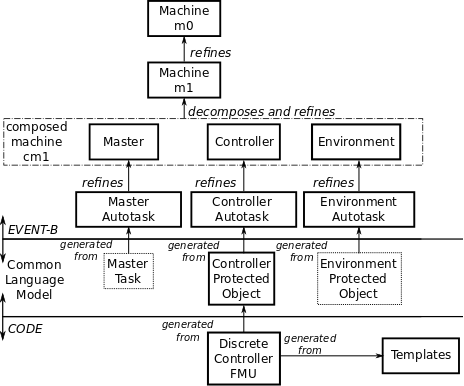
\includegraphics[width=0.7\textwidth]{devel.png}
\caption{The Code Generation Process}
\label{fig:CGProcess}
\vspace*{-12pt}
\end{figure}
The code generation phase (below this line) is a two-step process; although only a single step is visible to the user. The first step is to translate the Event-B machine to a language-neutral model, the Common Language Model (CLM). During the second step, when the source code is being generated, the templates contribute to the generated code. 

\section{Using Templates}\label{templates}
An architectural overview of our template-driven approach can be seen in the diagram of Fig.~\ref{fig:templates}.
%
\begin{figure}
\vspace*{-12pt}
\centering
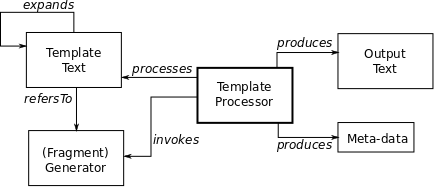
\includegraphics[width=0.6\textwidth]{templateOverview.png}
\caption{The Template Processor and Artefacts}
\label{fig:templates}
\vspace*{-5pt}
\end{figure}
%
We see the artefacts involved in template processing; namely text-based templates, code-fragment generators, text output, meta-data output and a template-processor that does the work. The templates may contain plain-text (which is copied verbatim to the target during processing) and tags. The tags may refer to other templates, or code-fragment generators. The code-fragment generators are hard-coded generators that relate to certain aspects of the final output; for instance, a fragment generator inserts the variable initialisations as specified in a template. We can see an example of this in Fig.~\ref{fig:templateExample}. 
%
\begin{figure}
\begin{center}
\begin{minipage}{0.6\textwidth}
\vspace*{-5pt}
\begin{spacing}{0.8}
\small
//\#\# $<$addToHeader$>$\\
fmiStatus fmiInitializeSlave(fmiComponent c,\\
\hspace*{0.2cm}fmiReal relativeTolerance, fmiReal tStart,\\
\hspace*{0.2cm}fmiBoolean stopTimeDefined, fmiReal tStop)\{\\
\hspace*{0.4cm}fmi\_Component* mc = c;\\
\hspace*{0.4cm}//\#\# $<$initialisationsList$>$\\
\hspace*{0.4cm}//\#\# $<$stateMachineProgramCounterIni$>$\\
\hspace*{0.4cm}return fmiOK;\\
\}
\normalsize
\end{spacing}
\caption{An Example Template}
\label{fig:templateExample}
\vspace*{-5pt}
\end{minipage}
\end{center}
\end{figure}
%
%
The template shows part of an implementation of the FMI API's \emph{fmiInitializeSlave} function; the code in the template is common to all of the FMUs that we will generate for a particular target configuration. The tags accommodate variability between models; e.g. FMUs keep track of state-variables, which may be different for each model. These state-variables correspond exactly to the variables of the system that have been modelled in Event-B. In the function shown, the first parameter is the \emph{fmiComponent}, the `instance' of the FMU that is to be initialised. The other parameters relate to the simulation life-cycle.  
In the template, we insert a place-holder (which we call a \emph{tag}), where we want variable initialisation to occur. The tags in our example begin with the character string, //\#\#.  The line continues with an \emph{identifier}, $<$\emph{identifier}$>$. A tag is usually (but not always) used as an insertion point; its \emph{identifier} can relate to another template (to be expanded and processed in-line); or the name of a fragment-generator. The fragment-generator is a Java class that can be used to generate code; or meta-data that is stored for later use, in the code generation process  (see Fig.~\ref{fig:templates}). In the example we have three tags. The first tag \emph{addToHeader} identifies a generator that creates meta-data, which are used at a later stage, for generation of a header file.

It is possible to categorize the users of Rodin into several types of users. One such type are the `ordinary' modellers, using Event-B in smaller organisations. But for large scale use, one may have meta-modellers (to develop product lines for instance), and another level of user may instantiate models (of the product line). There may also be platform developers, that provide platform tools for use by meta-modellers, modellers and product-line implementers. The extension points allow the platform developer to provide template utilities for the other users. They can define new tags and fragment-generators.
An overview of the  templates and generators used in the FMI translation, can be seen in Fig.~\ref{fig:templateStructure} (much of the detail is omitted for brevity). The \emph{root} template is \emph{fmuTemplate.c}, from this we can navigate to all of the other templates, and generators. The root template generates variable declarations and the subroutines, and expands the main boilerplate functions in \emph{fmuOthers.c}. The \emph{fmuInstantiate} and \emph{fmuInitialise} templates generate the corresponding FMI API function implementations. From the diagram we can see that these rely on generators to do some of the translation.
%
\begin{figure}[t]
\vspace*{-12pt}
\centering
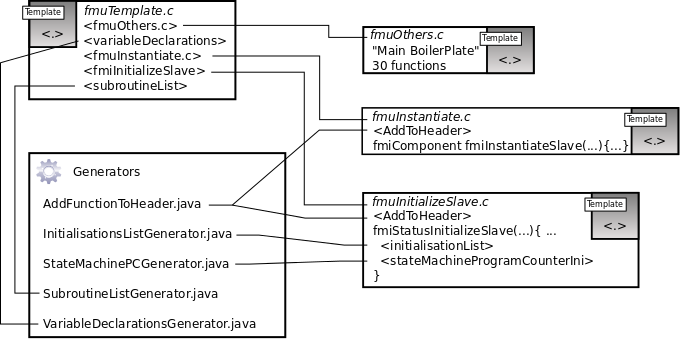
\includegraphics[width=0.8\textwidth]{templateStructure.png}
\caption{The Templates and Generators in the FMI Code Generator}
\label{fig:templateStructure}
\vspace*{-12pt}
\end{figure}
%
The template-processor scans each line, and copies the output; or inserts new text, or meta-data as required, until we reach a generator tag. The class's \emph{generate} method is invoked, to begin the process of text insertion. A fragment of the \emph{InitialisationListGenerator} class can be seen in Fig.~\ref{fig:genCode}. 
%
%
\begin{figure}[t]
\centering
\begin{minipage}{0.95\textwidth}
\begin{spacing}{0.8}
\small
\textbf{public class} InitialisationsListGenerator \textbf{implements} IGenerator \{\\
\hspace*{0.2cm}\textbf{public} List$<$String$>$ generate(IGeneratorData data)\{\\
\hspace*{0.4cm}List$<$String$>$ outCode = \textbf{new} ArrayList$<$String$>$();\\
\hspace*{0.4cm}Protected prot = null;\\
\hspace*{0.4cm}IL1TranslationManager tm = null;\\
\hspace*{0.4cm}\emph{//(1) Un-pack the GeneratorData}\\
\hspace*{0.4cm}List$<$Object$>$ dataList = data.getDataList();\\
\hspace*{0.4cm}\textbf{for} (Object obj : dataList) \{\\
\hspace*{0.6cm}\textbf{if} (obj instanceof Protected) \{prot = (Protected) obj;	\}\\
\hspace*{0.6cm}\textbf{else if}(obj instanceof IL1TranslationManager)\{\\
\hspace*{0.8cm}tm = (IL1TranslationManager) obj;\}\}\\
\hspace*{0.2cm}\ldots\\
\hspace*{0.2cm}\emph{//(2) Get the Declarations}\\
\hspace*{0.2cm}EList$<$Declaration$>$ declList = prot.getDecls();\\
\hspace*{0.2cm}\emph{//(3) Process each Variable Declaration/Initialisation}\\
\hspace*{0.2cm}\textbf{for} (Declaration decl : declList) \{\\
\hspace*{0.4cm}\ldots\\
\hspace*{0.4cm}String initialisation = FMUTranslator.updateFieldVariableName(\ldots);\\
\hspace*{0.4cm}outCode.add(initialisation);\\
\hspace*{0.2cm}\}\\
\hspace*{0.2cm}\emph{// (4) return the new fragment}\\
\hspace*{0.2cm}\textbf{return} outCode;\}\}
\normalsize
\end{spacing}
\end{minipage}
\caption{An Example Fragment-Generator}
\label{fig:genCode}
\end{figure}
%
%
The main steps are highlighted using numbered comments in the code. In step 1, the data is un-packed; in step 2, the declarations are obtained from the \emph{Protected} object; in step 3, the initialisation are translated, and add to an array of initialisation statements; in step 4, the initialisations are returned to the template-processor. 
%
\section{Conclusions}\label{conc}
Using the approach that we have described in this paper, we are able to perform target configuration prior to code-generation; and re-use boilerplate code, without having to hard-code it. The template-processor reads each line of a template and copies the contents, verbatim, to a target file unless a template tag is encountered. A tag can refer to another template, which is processed by expanding it in-line, or a custom fragment generator. As part of an extensible approach, a platform developer can enrich the template language, by adding new template tags and associate them with custom fragment-generators. In this way complex code generation activities can be performed, to generate text output, or  to generate meta-data in other formats. The meta-data is useful for downstream code generation. We used the template-driven approach to implement part of a new code generator, translating Event-B models to FMI-C code. 
%
\bibliographystyle{plain}
\bibliography{MyBibTex}
%
%
%
\end{document}
